\chapter{U-Prove\label{chp:uprove}}

Stefan Brands provided the first integral description of the U-Prove technology
in his thesis~\cite{Brands2000}, after which he founded the company Credentica
to implement and sell this technology. Microsoft acquired Credentica and
published the U-Prove cryptographic specification~\cite{U-Prove_Crypto2010,
U-Prove_Crypto2013} under the Open Specification Promise\footnote{%
\url{http://www.microsoft.com/interop/osp/}} together with open source reference
software development kits in C\# and Java.

The U-Prove technology is centred around a so-called U-Prove token. This token
serves as a pseudonym for the user. It contains a number of attributes which can
be selectively disclosed to a verifier. Hence the user decides which attributes
to show and which to withhold (for example, one can reveal the birth date, but
not the residence address). Finally there is the token's public-key, which
aggregates all information in the token, and a signature from the issuer over
this public-key to ensure the authenticity.

A previous attempt to implement this technology on a smart card by Tews and
Jacobs~\cite{TewsJacobs09}, based on Brands' description~\cite{Brands2000},
resulted in a highly involved Java Card applet with running times in the order
of 5--10 seconds which make it not really usable in practice. They concluded
that the lack of cryptographic hardware support through the Java Card API was
the main cause of the slow performance. Therefore, we decided to develop our
application using the MULTOS platform, which offers a much more suitable API.
Our implementation, which we describe in Section~\ref{sec:UP-smartcard}, not
only has a much better performance but is also, except from some minimal
limitations, compatible with the development kits released by Microsoft.

\section{Schnorr Signature Scheme}

The Schnorr signature scheme~\cite{Schnorr1989,Schnorr1991} relies on the
Schnorr identification protocol~\cite{Schnorr1989} which is a special instance
of the interactive protocol of Chaum, Evertse and Van de
Graaf~\cite{ChaumEvdG1988} that proves knowledge of a discrete logarithm key
pair. It is derived from this identification scheme by replacing the verifier's
challenge by a hash value according to the Fiat-Shamir
heuristic~\cite{FiatShamir1987} as can be seen in
Algorithm~\ref{alg:Schnorr-sign}.

\begin{algorithm}
  \caption{Generate a Schnorr signature.}
  \label{alg:Schnorr-sign}
  \addtolength{\baselineskip}{1mm}
  \begin{algorithmic}[1]
    \Function{Schnorr-sign}{$m, (p, q, g), x$}
      \State $u \gets \Call{Random}{~}$
      \State $a \gets g^u \mod p$
      \State $c \gets \Call{Hash}{a, m}$
      \State $r \gets u + c \cdot x \mod q$

      \Return $(c, r)$
    \EndFunction
  \end{algorithmic}
\end{algorithm}
\begin{algorithm}
  \caption{Verify a Schnorr signature.}
  \label{alg:Schnorr-verify}
  \addtolength{\baselineskip}{1mm}
  \begin{algorithmic}[1]
    \Function{Schnorr-verify}{$(c, r), m, (p, q, g), h$}
      \State $\hat{a} \gets g^r \cdot h^{-c} \mod p$

      \If{$c \neq \Call{Hash}{\hat{a}, m}$}
        \Return \Call{Invalid}{}
      \EndIf

      \Return \Call{Valid}{}
    \EndFunction
  \end{algorithmic}
\end{algorithm}

The private key is a random value $x$. The corresponding public key is a value
$h = g^x \mod p$ together with a description of the prime-order group in which
the computations take place. As an example we use $(p, q, g)$, which denotes a
subgroup of $\Z^*_p$ of prime-order $q$ with generator $g$. The signature over
a message $m$ is the resulting pair $(c, r)$.

Verification of such a Schnorr signature $(c, r)$ starts with the reconstruction
of the input value for the hash function based on $r$, according to the
following equation:
\begin{equation}\label{eqn:Schnorr-verify}
  \hat{a} = g^r \cdot h^{-c} = g^{u + c \cdot x} \cdot g^{-c \cdot x} = g^u = a \mod p
\end{equation}
If the signature is valid, that is, this equation holds, the resulting output of
the hash function matches $c$ (see Algorithm~\ref{alg:Schnorr-verify}).

\subsection{Blind Signatures}

\begin{figure}[ht]
  \centering
  \includegraphics[scale=.45]{mscs/schnorr_blind-sign}
  \caption{Protocol for generating blind signatures.}
  \label{msc:schnorr_blind-sign}
\end{figure}

Figure~\ref{msc:schnorr_blind-sign} depicts the protocol for generating blind
signatures~\cite{PointchevalStern1996}. The steps executed by the signer are
similar to the original signing protocol. In Algorithm~\ref{alg:Schnorr-prepare}
the signer constructs a commitment $a$, to the randomisation value $u$, which is
sent to the recipient of the signature.

The recipient generates blinding values $v$ and $w$ to hide the message $m$ that
it whats to get signed. A (blinded) commitment $c$ to this message is generated
(see Algorithm~\ref{alg:Schnorr-commit}) and sent to the signer.

\begin{algorithm}[H]
  \caption{Prepare for a blind Schnorr signature.}
  \label{alg:Schnorr-prepare}
  \addtolength{\baselineskip}{1mm}
  \begin{algorithmic}[1]
    \Function{Schnorr-prepare}{$(p, q, g)$}
      \State $u \gets \Call{Random}{~}$
      \State $a \gets g^u \mod p$

      \Return $a, u$
    \EndFunction
  \end{algorithmic}
\end{algorithm}

\begin{algorithm}
  \caption{Commit to the message for a blind Schnorr signature.}
  \label{alg:Schnorr-commit}
  \addtolength{\baselineskip}{1mm}
  \begin{algorithmic}[1]
    \Function{Schnorr-commit}{$m, a, (p, q, g)$}
      \State $v \gets \Call{Random}{~}$
      \State $w \gets \Call{Random}{~}$
      \State $a' \gets a \cdot g^v \cdot h^w \mod p$
      \State $c' \gets \Call{Hash}{a', m}$
      \State $c \gets c' + w \mod q$
      \Return $c, c', v$
    \EndFunction
  \end{algorithmic}
\end{algorithm}

Upon receipt of the message commitment, the signer constructs the Schnorr
signature value $r$ according to Algorithm~\ref{alg:Schnorr-blind-sign} and
returns this value to the recipient. Finally, the recipient checks whether the
received value is correct according to (\ref{eqn:Schnorr-verify}) and computes
the last element of the blind Schnorr signature $(c', r')$.

The resulting signature $(c', r')$ can then be verified using the regular
verification procedure, Algorithm~\ref{alg:Schnorr-verify}. This works since:
\begin{align*}
  \hat{a}
  & = g^{r'} \cdot h^{-c'}
  = g^{r + v} \cdot g^{-c' \cdot x}
  = g^{u + c \cdot x + v} \cdot g^{-c' \cdot x}
  = g^{u + (c' + w) \cdot x + v} \cdot g^{-c' \cdot x} \\
  & = g^u \cdot g^v \cdot g^{c' \cdot x} \cdot g^{w \cdot x} \cdot g^{-c' \cdot x}
  = g^u \cdot g^v \cdot g^{x \cdot w}
  = a \cdot g^v \cdot h^w
  = a' \mod p
\end{align*}

\begin{algorithm}[H]
  \caption{Generate a blind Schnorr signature.}
  \label{alg:Schnorr-blind-sign}
  \addtolength{\baselineskip}{1mm}
  \begin{algorithmic}[1]
    \Function{Schnorr-blind-sign}{$c, u, (p, q, g), x$}
      \State $r \gets u + c \cdot x \mod q$

      \Return $r$
    \EndFunction
  \end{algorithmic}
\end{algorithm}
\begin{algorithm}
  \caption{Finish a blind Schnorr signature.}
  \label{alg:Schnorr-finish}
  \addtolength{\baselineskip}{1mm}
  \begin{algorithmic}[1]
    \Function{Schnorr-finish}{$r, a, c, c', v, (p, q, g), h$}
      \State $\hat{a} \gets g^r \cdot h^{-c} \mod p$
      \If{$a \neq \hat{a}$}
        \Return \Call{Invalid}{}
      \EndIf

      \State $r' \gets r + v \mod q$

      \Return $(c', r')$
    \EndFunction
  \end{algorithmic}
\end{algorithm}

\section{U-Prove Credentials}

The U-Prove technology is built around U-Prove tokens. These tokens are in
principle a collection of attributes signed by an issuer. The issuer's public
key $(g_0, \{g_i\}_{i \in \A})$ consists of a value $g_0 = g^x \mod p$ which
commits to the private key $x$ and a random generator $g_i$ for each possible
attribute ($\A$ denotes the set of attribute indices).

In order for the attributes $\{a_i\}_{i \in \A}$, to be signed they are
aggregated into what is called the token public key $h = h'^s \mod p$ where $s$
is the user's secret and $h'$ is the aggregation of the attributes using the
issuer's public key:
\begin{equation}\label{eqn:UP-attribute-aggregation}
  h' = g_0 \cdot \textstyle\prod_{i \in \A} g_i^{a_i} \mod p
\end{equation}
The corresponding token private key $s' = s^{-1} \mod q$. Together with the
issuer's signature $(z', c', r')$, generated during the issuance process (see
Section~\ref{sec:UP-issuance}), these values form a U-Prove token. Such a token
serves as a pseudonym for the user. A collection of U-Prove tokens, where only
the signatures differ, can be seen as a U-Prove credential.

A U-Prove credential usually consist of multiple tokens to achieve anonymity,
since a single token acts as a pseudonym for the user. This means that whenever
the user does not want to be traced during a credential verification (see
Section~\ref{sec:UP-verification}) she should use a fresh token to prevent the
verifier from linking the token to previous transactions.

To summarise, a U-Prove credential, as depicted in
Figure~\ref{fig:uprove-credential}, consists of:
\begin{itemize}
  \item a collection of attributes $\{a_i\}_{i \in \mathcal{A}}$ aggregated in $h'$,
  \item a key pair ($h = h'^s \mod p$, $s' = s^{-1} \mod q$), based on the user's secret~$s$, and
  \item a number of signatures $(z', c', r')$, over the token public key (and hence over the user's secret and the attributes).
\end{itemize}
\begin{figure}[H]
  \centering
  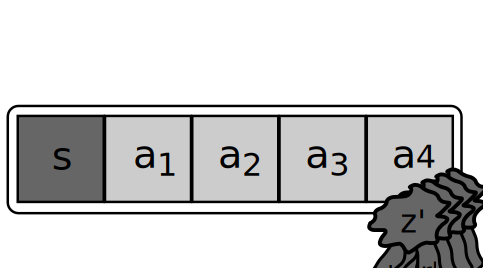
\includegraphics[scale=.45]{images/uprove-credential}
  \caption{A visual representation of a U-Prove credential.}
  \label{fig:uprove-credential}
\end{figure}

\section{Credential Issuance}\label{sec:UP-issuance}

\begin{figure}[ht]
  \centering
  \includegraphics[scale=.45]{mscs/uprove-issuance}
  \caption{Protocol for U-Prove credential issuance.}
  \label{msc:uprove-issuance}
\end{figure}

Figure~\ref{msc:uprove-issuance} depicts the issuance protocol for a U-Prove
token. The issuer starts by computing $z = h'^x \mod p$ which combines its
private key $x$ with the attributes $a_{i \in \A}$, aggregated according to
(\ref{eqn:UP-attribute-aggregation}). Next, the issuer commits to the
randomisation value $u$ using both the generator $g$ and the aggregated
attributes $h'$ that are going to be signed (see
Algorithm~\ref{alg:UP-issuance-prepare}).

\begin{algorithm}
  \caption{Prepare for U-Prove issuance.}
  \label{alg:UP-issuance-prepare}
  \addtolength{\baselineskip}{1mm}
  \begin{algorithmic}[1]
    \Function{UP-issuance-prepare}{$h', (p, q, g), x$}
      \State $z \gets h'^x \mod p$

      \State $u \gets \Call{Random}{~}$
      \State $a \gets g^u \mod p$
      \State $b \gets h'^u \mod p$

      \Return $z, a, b, u$
    \EndFunction
  \end{algorithmic}
\end{algorithm}

The user starts in Algorithm~\ref{alg:UP-issuance-commit} by generating a fresh
secret $s$ and computes the token private key $s'$. She then combines this
secret with the aggregated attributes $h'$ and the value $z$, received from the
issuer, to obtain, respectively, the token public key and the first element of
the signature $z'$. The remaining steps compute the commitment to these values
similar to Schnorr's blind signature scheme (Algorithm~\ref{alg:Schnorr-commit}).

\begin{algorithm}
  \caption{Commit to the attributes for U-Prove issuance.}
  \label{alg:UP-issuance-commit}
  \addtolength{\baselineskip}{1mm}
  \begin{algorithmic}[1]
    \Function{UP-issuance-commit}{$h', z, a, b, (p, q, g)$}
      \State $s \gets \Call{Random}{~}$
      \State $s' \gets s^{-1} \mod q$
      \State $h \gets h'^s \mod p$
      \State $z' \gets z^s \mod p$

      \State $v \gets \Call{Random}{~}$
      \State $w \gets \Call{Random}{~}$
      \State $a' \gets a \cdot g^v \cdot g_0^w \mod p$
      \State $b' \gets b^s \cdot h^v \cdot z'^w \mod p$

      \State $c' \gets \Call{Hash}{h, z', a', b'} \mod q$
      \State $c \gets c' + w \mod q$

      \Return $z', a', b', c, c', v, s'$
    \EndFunction
  \end{algorithmic}
\end{algorithm}

The issuer then performs the next step of Schnorr's blind signature scheme
(Algorithm~\ref{alg:Schnorr-blind-sign}) and signs the commitment $c$ received
from the user according to Algorithm~\ref{alg:UP-issuance-sign}.

\begin{algorithm}
  \caption{Sign the attributes for U-Prove issuance.}
  \label{alg:UP-issuance-sign}
  \addtolength{\baselineskip}{1mm}
  \begin{algorithmic}[1]
    \Function{UP-issuance-blind-sign}{$c, u, (p, q, g), x$}
      \State $r \gets u + c \cdot x \mod q$

      \Return $r$
    \EndFunction
  \end{algorithmic}
\end{algorithm}

Finally, in Algorithm~\ref{alg:UP-issuance-finish}, the user computes $r'$, the
last element of the token signature $(z', c', r')$. Using this value she can
also verify whether the values received from the issuer are correct:
\begin{align*}
  a' \cdot b'
  & = a' \cdot b' \cdot g_0^{c'} \cdot g_0^{-c'} \cdot h^{c' \cdot x} \cdot h^{-c' \cdot x} \\
  & = a \cdot g^v \cdot g_0^w \cdot b^s \cdot h^v \cdot z'^w
    \cdot g_0^{c'} \cdot g_0^{-c'} \cdot h^{c' \cdot x} \cdot h^{(-c + w) \cdot x} \\
  & = g^u \cdot g^v \cdot g_0^w \cdot h'^{u \cdot s} \cdot h^v \cdot z^{s \cdot w}
    \cdot g_0^{c'} \cdot g_0^{-c'} \cdot h^{c' \cdot x} \cdot h^{-c \cdot x} \cdot h^{w \cdot x} \\
  & = g^u \cdot g^v \cdot g^{w \cdot x} \cdot h^u \cdot h^v \cdot z^{w \cdot s}
    \cdot g^{c' \cdot x} \cdot g_0^{-c'}  \cdot h^{c' \cdot x} \cdot h^{w \cdot x} \cdot z^{-c \cdot s} \\
  & = g^u \cdot g^{c' \cdot x} \cdot g^{w \cdot x} \cdot g^v \cdot h^u
    \cdot h^{c' \cdot x} \cdot h^{w \cdot x} \cdot h^v \cdot g_0^{-c'} \cdot z^{-c \cdot s} \cdot z^{w \cdot s} \\
  & = g^{u + c' \cdot x + w \cdot x + v} \cdot h^{u + c' \cdot x + w \cdot x + v}
    \cdot g_0^{-c'} \cdot z^{(-c + w) \cdot s} \\
  & = (g \cdot h)^{u + c' \cdot x + w \cdot x + v} \cdot g_0^{-c'} \cdot z'^{-c + w} \\
  & = (g \cdot h)^{u + c \cdot x + v} \cdot g_0^{-c'} \cdot z'^{-c + w} \\
  & = (g \cdot h)^{r + v} \cdot g_0^{-c'} \cdot z'^{-c'} \\
  & = (g \cdot h)^{r'} \cdot (g_0 \cdot z')^{-c'} \mod p
\end{align*}

\begin{algorithm}
  \caption{Finish U-Prove issuance.}
  \label{alg:UP-issuance-finish}
  \addtolength{\baselineskip}{1mm}
  \begin{algorithmic}[1]
    \Function{UP-issuance-finish}{$a', c', z', v, r, (p, q, g), h$}
      \State $r' \gets r + v \mod q$

      \If{$a' \cdot b' \neq (g \cdot h)^{r'} \cdot (g_0 \cdot z')^{-c'}$}
        \Return \Call{Invalid}{}
      \EndIf

      \Return $(z', c', r')$
    \EndFunction
  \end{algorithmic}
\end{algorithm}

\section{Credential Verification}\label{sec:UP-verification}

\begin{figure}[ht]
  \centering
  \includegraphics[scale=.45]{mscs/uprove-verification}
  \caption{Protocol for U-Prove credential verification.}
  \label{msc:uprove-verification}
\end{figure}

The verification of a U-Prove credential consists of two parts. First, the
verifier must check whether the signature over the token public key is valid. To
this end the user sends the token public key and signature to the verifier as
can be seen in Figure~\ref{msc:uprove-issuance}.
\begin{algorithm}
  \caption{Verify a U-Prove token signature.}
  \label{alg:UP-verify-token}
  \addtolength{\baselineskip}{1mm}
  \begin{algorithmic}[1]
    \Function{UP-verify-token}{$h, (z', c', r'), (p, q, g)$}
      \State $\hat{a} \gets g^{r'} \cdot g_0^{-c'} \mod p$
      \State $\hat{b} \gets h^{r'} \cdot z'^{-c'} \mod q$
      \If{$c' \neq \Call{Hash}{h, z', \hat{a}, \hat{b}}$}
        \Return \Call{Invalid}{}
      \EndIf

      \Return $\Call{Valid}{}$
    \EndFunction
  \end{algorithmic}
\end{algorithm}

The verifier can then verify the validity of the signature $(z', c', r')$ using
Algorithm~\ref{alg:UP-verify-token}. Similar to the Schnorr signature
verification, the verifier reconstructs the input values $\hat{a}$ and
$\hat{b}$ for the hash function according to the following equations:
\begin{align*}
  \hat{a}
  & = g^{r'} \cdot g_0^{-c'}
  = g^{r + v} \cdot g^{-c' \cdot x}
  = g^{u + c \cdot x + v} \cdot g^{-c' \cdot x}
  = g^{u + (c' + w) \cdot x + v} \cdot g^{-c' \cdot x} \\
  & = g^u \cdot g^{c' \cdot x} \cdot g^{w \cdot x} \cdot g^v \cdot g^{-c' \cdot x}
  = g^u \cdot g^{w \cdot x} \cdot g^v
  = g^u \cdot g^v \cdot g_0^w
  = a \cdot g^v \cdot g_0^w \\
  & = a' \mod p
\end{align*}

\begin{align*}
  \hat{b}
  & = h^{r'} \cdot z'^{-c'}
  = h^{u + c \cdot x + v} \cdot z^{-c' \cdot s}
  = h^{u + (c' + w) \cdot x + v} \cdot h'^{-c' \cdot s \cdot x} \\
  & = h^u \cdot h^{c' \cdot x} \cdot h^{w \cdot x} \cdot h^v \cdot h^{-c' \cdot x}
  = h^u \cdot h^v \cdot h'^{s \cdot w \cdot x}
  = h'^{u \cdot s} \cdot h^v \cdot z^{s \cdot w}
  = b^s \cdot h^v \cdot z'^w \\
  & = b' \mod p
\end{align*}

If the signature is valid, that is, both equations hold, the resulting output of
the hash function matches $c'$.

The second part of the credential verification protocol of
Figure~\ref{msc:uprove-verification} consists of selective disclosure of the
attributes and a proof of knowledge of the token private key. In this part the
user sends the disclosed attributes $\{a_i\}_{i \in \A_D}$, where $\A_D$ is the
set of disclosed attribute indices, to the verifier and includes the undisclosed
attributes in the proof of knowledge of the token private key. This proof of
knowledge can be generated using Algorithm~\ref{alg:UP-selective-disclosure}.
The freshness of this proof is guaranteed by a nonce $n_D$ provided by the
verifier.

\begin{algorithm}
  \caption{U-Prove selective disclosure.}
  \label{alg:UP-selective-disclosure}
  \addtolength{\baselineskip}{1mm}
  \begin{algorithmic}[1]
    \Function{UP-selective-disclosure}{$\{a_i\}_{i \in \A}, h, (z', c', r'), s', n_D, (p, q, g)$}
      \State $\tilde{s} \gets \Call{Random}{~}$
      \State $a \gets h^{\tilde{s}} \mod p$
      \ForAll{$i \in \A \setminus \A_D$}
        \State $\tilde{a}_i \gets \Call{Random}{~}$
        \State $a \gets a \cdot g_i^{\tilde{a}_i} \mod p$
      \EndFor
      \State $c' \gets \Call{Hash}{a}$

      \State $c \gets \Call{Hash}{c, a_{i \in \A_D}, n_D} \mod q$

      \State $\hat{s} \gets \tilde{s} + c \cdot s' \mod q$
      \ForAll{$i \in \A \setminus \A_D$}
        \State $\hat{a}_i \gets \tilde{a}_i - c \cdot a_i \mod q$
      \EndFor

      \Return $\{a_i\}_{i \in \A_D}, \{\hat{a}_i\}_{i \in \A \setminus \A_D}, c', \hat{s}$
    \EndFunction
  \end{algorithmic}
\end{algorithm}

\begin{algorithm}
  \caption{U-Prove proof verification.}
  \label{alg:UP-verify-proof}
  \addtolength{\baselineskip}{1mm}
  \begin{algorithmic}[1]
    \Function{UP-verify-proof}{$\{a_i\}_{i \in \A_D}, \{\hat{a}_i\}_{i \in \A \setminus \A_D}, c', \hat{s}, n_D, (p, q, g)$}
      \State $c \gets \Call{Hash}{c', a_{i \in \A_D}, n_D}$
      \State $\hat{a} \gets g_0^{-c} \cdot h^{\hat{s}} \mod p$

      \ForAll{$i \in \A_D$}
        \State $\hat{a} \gets \hat{a} \cdot g_i^{-c \cdot a_i} \mod p$
      \EndFor
      \ForAll{$i \in \A \setminus \A_D$}
        \State $\hat{a} \gets \hat{a} \cdot g_i^{\hat{a}_i} \mod p$
      \EndFor

      \If{$c' \neq \Call{Hash}{\hat{a}}$}
        \Return \Call{Invalid}{}
      \EndIf

      \Return \Call{Valid}{}
    \EndFunction
  \end{algorithmic}
\end{algorithm}

The selective disclosure proof can be verified using
Algorithm~\ref{alg:UP-verify-proof}. The verification succeeds if the verifier
can successfully reconstruct the commitment $a$ generated by the user. This
reconstruction works because of the following equation:
\begin{align*}
  \hat{a}
  & = g_0^{-c} \cdot h^{\hat{s}}
    \cdot \textstyle\prod_{i \in \A_D} g_i^{-c \cdot a_i}
    \cdot \textstyle\prod_{i \in \A \setminus \A_D} g_i^{\hat{a}_i} \\
  & = g_0^{-c} \cdot h^{\tilde{s} + c \cdot s'}
    \cdot \textstyle\prod_{i \in \A_D} g_i^{-c \cdot a_i}
    \cdot \textstyle\prod_{i \in \A \setminus \A_D} g_i^{\tilde{a}_i - c \cdot a_i} \\
  & = g_0^{-c} \cdot h^{\tilde{s}} \cdot h^{c \cdot s'}
    \cdot \textstyle\prod_{i \in \A_D} g_i^{-c \cdot a_i}
    \cdot \textstyle\prod_{i \in \A \setminus \A_D} g_i^{\tilde{a}_i}
    \cdot \textstyle\prod_{i \in \A \setminus \A_D} g_i^{- c \cdot a_i} \\
  & = g_0^{-c} \cdot h^{\tilde{s}} \cdot h'^{c \cdot s' \cdot s}
    \cdot \textstyle\prod_{i \in \A} g_i^{-c \cdot a_i}
    \cdot \textstyle\prod_{i \in \A \setminus \A_D} g_i^{\tilde{a}_i} \\
  & = h^{\tilde{s}} \cdot h'^{c} \cdot h'^{-c}
    \cdot \textstyle\prod_{i \in \A \setminus \A_D} g_i^{\tilde{a}_i} \\
  & = h^{\tilde{s}}
    \cdot \textstyle\prod_{i \in \A \setminus \A_D} g_i^{\tilde{a}_i} \\
  & = a \mod p
\end{align*}


\section{U-Prove on Smart Cards}\label{sec:UP-smartcard}

The use of U-Prove in combination with a smart card was already envisioned by
Brands~\cite{Brands2000} and published by Microsoft in version~1.1 of the
U-Prove cryptographic specification~\cite{U-Prove_Crypto2011}. Their idea is to
use a smart card (or even any trusted computing device) as a manner of
protecting U-Prove tokens, which they then call device-protected tokens. This is
achieved by having the device contribute one attribute to the token. The actual
value of this attribute is, like a private key, only known by the device and
will always be hidden. Therefore the device is required during the verification
protocol, since the user has to prove knowledge of \emph{all} undisclosed
attributes.

Besides adding an additional layer of protection the U-Prove technology
overview~\cite{U-Prove_Overview2011} describes a number of other benefits
gained when using device-protected tokens. For example, a device can be used to
enforce dynamic policies or prevent the use of a token at a blacklisted website.
It also helps to enforce non-transferability of tokens by having the user
authenticate to the device before allowing it to be used in a transaction.
Another option, especially interesting for smart cards, is to use the device as
a carrier, or secure roaming store, for entire U-Prove credentials and not just
one attribute. This way the U-Prove credentials are always available when needed.

This last feature of a device-protected U-Prove token has one major drawback,
namely one will need to trust the device that is used to perform the proving
protocol. This is because the actual attribute values are used during the
computation steps of this protocol (see Section~\ref{sec:UP-verification}).
Hence the device must release all information, except its own special attribute,
during a protocol run. When using a personal computer this might be acceptable,
but in scenarios where the device should be used directly with a verifier, for
example at a public transport gate, or at a vending machine for cigarettes, this
turns out to be problematic. Since these are the areas of use which are most
interesting for us, we decided to develop an implementation which provides the
full verification protocol on a smart card instead of using Microsoft's more
limited approach.

\subsection{Smart Card Implementation}

A very general view of our implementation of the U-Prove technology is that it
provides storage for preloaded (e.g.\ cryptographic domain parameters) and
calculated (e.g.\ generated keys) values of the protocols, as well as attribute
storage, and, more importantly, a sequence of hash and modulo prime arithmetic
operations to execute the corresponding stages of the protocols. These
arithmetic operations are the core of the performance considerations of our
implementation. A few hashing operations are executed and multiple exponents
over numbers in a large prime field have to be calculated during a verification
protocol run.

Considering the size of the U-Prove data that is used in the protocols and the
requirements of the MULTOS cryptographic routines (all data for a cryptographic
operation needs to be in one continuous array) the first thing to take care of
is a careful split of the card data between EEPROM and RAM. Only 960
\emph{bytes} of RAM are available on our development cards, compared to
36 \emph{kilo}bytes of EEPROM. The most frequent use case of the card is the
execution of the proving protocol, hence this is where good use of RAM is highly
desirable. For that we limited the maximum number of stored attributes to 5 and
then we ensured that all variables used in the verification protocol are
allocated in RAM.

The initialisation and issuance protocol require more scratch-pad memory than
the available RAM, hence we were forced to use EEPROM there. Moreover, the
issuance protocol makes use of EEPROM for permanent storage of the issued
U-Prove token and other permanent protocol parameters (prime numbers $p$, $q$,
etc.). The use of EEPROM for computations has an impact on the running time for
these operations, as can be seen in Section~\ref{sec:UP-performance}, but this
is acceptable given that these operations are normally only used a limited
number of times.

This completes the efficiency considerations for our implementation. Otherwise
the implementation of the U-Prove protocols is rather straightforward in the
MULTOS environment and mostly entails direct calls to the MULTOS API.

\subsection{Integration into the Microsoft U-Prove SDK}

The previous section described the implementation of the U-Prove protocols which
mainly concerns storage and the mathematical computations. This is, however, not
sufficient to use it in combination with Microsoft's U-Prove software
development kit. We need to bridge between the high-level Java interfaces
defined in this development kit and the low-level APDU interface of the smart
card.

We designed the low-level APDU interface to be as simple as possible.
Essentially it has to provide three types of functionality:
\begin{enumerate}
  \item sending data to the card,
  \item ask the card to perform the necessary computations, and
  \item retrieve the results from the card.
\end{enumerate}
The second type of the interface functionality is easiest, we just defined an
APDU instruction for each of the steps in the protocols. For transferring data
to and from the card we restricted the values to the maximum amount of data that
can be transferred in one APDU (255 bytes). This allows us to just define one
APDU instruction per variable, parametrised only with the index if needed (for
example $g_i$), for setting or getting a value.

Finally we need to bind this low level APDU API to the interfaces and data types
provided by the U-Prove software development kit. Luckily the development kit
just uses byte arrays for the external access to the data types such that no
additional conversion is needed. The only thing that needs to be done for a data
type, for example \texttt{IssuerParameters}, is that the setter and getter
have to be divided into the individual APDU instructions, for example the
\texttt{setPublicKey} and \texttt{setEncodingBytes} instructions.

All this functionality has been combined into a single Java class which provides
setters and getters for the data stored on the card as well as methods for the
protocol steps. Using the Java built-in smart card library it serves as an
interface between our MULTOS implementation and the U-Prove software development
kit.

\section{Performance Results\label{sec:UP-performance}}

The two most important factors for us to test in our U-Prove implementation were
correctness of the protocol calculations (obviously) and the speed. Testing the
correctness was fairly easy. Since we interfaced our card to Microsoft's U-Prove
SDK we could simply test it by invoking the protocol runs from the SDK and check
the results. During the first stages of the development partial protocol
calculations were verified with the test vectors provided with the U-Prove
SDK~\cite{U-Prove_Vectors2011}. In the whole process a few corner case problems
with our calculations surfaced that required minor corrections.

For the performance tests we are restricted by the limits of our MULTOS
implementation platform. Namely, on our development cards we are limited to a
modulus size of 1024~bits for modular arithmetic,\footnote{The card actually
supports up to 2048~bits, but then during exponentiation only small enough
exponents can be used, a requirement which the U-Prove operations do not
satisfy.} and SHA-1 is the only built-in hashing algorithm available. Although
this may sound restrictive, it also makes the choice of the U-Prove protocol
configuration (protocol parameters) for our tests easy. We have simply chosen to
use the domain parameters fixed to the same ones as in the default configuration
of the official U-Prove SDK reference implementation and official U-Prove test
vectors~\cite{U-Prove_Vectors2011}, that is 1024~bits for modulus size and SHA-1
for hashing to match with the capabilities of the card.

\begin{figure}
  \centering
  \includegraphics{images/uprove-issuance.mps}
  \caption[Credential issuance times.]{
    Credential issuance times
    (\raisebox{-.8\dp\strutbox}{\includegraphics{images/box-dark.mps}}: computation,
      \raisebox{-.8\dp\strutbox}{\includegraphics{images/box-light.mps}}: overhead).}
  \label{fig:issue}
\end{figure}

As we stated in the previous section, for speed we concentrated our
implementation efforts on the every day use case of the application, that is,
the credential verification protocol. However, we also strived to optimise the
rest of the protocols to maintain speed also during the initialisation and
issuance parts. For the performance analysis, we executed a number of full
protocol runs (initialisation, issuance, proving) on the card in various
configurations. First of all we varied the number of stored attributes on the
card, then within this attribute range we varied the number of (un)disclosed
attributes. As shown in Figure~\ref{fig:issue} this resulted in a running time
of 3.6 and 5.5 seconds for the issuance of a U-Prove token with respectively 2
and 5 attributes. The dark grey area on the graph indicates the core running
time of the protocol calculations on the card, whereas light grey indicates the
remaining overhead. This overhead consists of transferring data to the card and
communicating the results of the protocol run between the card and PC.

\begin{figure}[hbt]
  \centering
  \begin{subfigure}[b]{0.4\textwidth}
    \includegraphics{images/uprove-2attr.mps}
    \caption{2 stored attributes}
    \label{fig:2attr}
  \end{subfigure}
  \begin{subfigure}[b]{0.5\textwidth}
    \includegraphics{images/uprove-4attr.mps}
    \caption{4 stored attributes}
    \label{fig:4attr}
  \end{subfigure}

  \vspace{5mm}

  \begin{subfigure}[b]{0.4\textwidth}
    \includegraphics{images/uprove-3attr.mps}
    \caption{3 stored attributes}
    \label{fig:3attr}
  \end{subfigure}
  \begin{subfigure}[b]{0.5\textwidth}
    \includegraphics{images/uprove-5attr.mps}
    \caption{5 stored attributes}
    \label{fig:5attr}
  \end{subfigure}

  \caption[Credential verification times for different configurations.]{
    Credential verification times for different configurations
    (\raisebox{-.8\dp\strutbox}{\includegraphics{images/box-dark.mps}}: computation,
      \raisebox{-.8\dp\strutbox}{\includegraphics{images/box-light.mps}}: overhead).}
  \label{fig:total}
\end{figure}

Correspondingly, the cumulative results for the attribute proving protocol are
shown in Figure~\ref{fig:total}. What can be seen in these graphs is that under
``full load'' our implementation executes the complete proving protocol in just
under 0.9 seconds (graph~\ref{fig:5attr}). In this worst-case scenario 5
attributes are stored on the card, none of which are disclosed during the
protocol run. In other words, the U-Prove token is only validated for its
authenticity without revealing any attributes. Such a scenario is not very
likely to occur in reality. In a more likely scenario at least one or two
attributes are going to be disclosed and we can also assume that a U-Prove token
will contain less attributes (or, that a large number of attributes can be split
into several separate U-Prove tokens). As the graphs show, reducing the number
of stored attributes improves the running time at a rate of 100 milliseconds per
attribute, and also that the performance increases along with increasing the
number of disclosed attributes, roughly 50 milliseconds per each extra disclosed
attribute. Overall, this brings the total execution time for a two attribute
token disclosing one attribute to under 0.5 seconds (graph~\ref{fig:2attr}).

One of the reasons to justify the Microsoft's device protected approach as
described in Section~\ref{sec:UP-smartcard} are possible resource issues with
smart cards (limited storage space and limited speed). Our performance results
undermine this argument. The worst case execution time of the proving part is
869 milliseconds. This not only makes the card implementation fast enough to be
usable in general, it also makes it usable for ``field'' applications, for
example dispensing machines. Even more, for smaller numbers of attributes the
running times become almost acceptable for use in public transport\slash
e-ticketing, where the commonly required card transaction times should stay
below 350 milliseconds. We also see a potential to improve the running times
using faster smart card hardware, we elaborate on this in the upcoming section.
Overall, these good results strongly justify the idea to use U-Prove standalone
on a smart card rather than to use Microsoft's device-protected token approach,
which now has no obvious functional or performance advantages over our approach.

The only limitations of our implementation are imposed by the limited resources
of the MULTOS smart card. We had to limit the prime modulus size to 1024 bits,
use only SHA-1 hashing, and because of the available RAM (less than 1kB) on the
card we could only allow for the maximum of 5 attributes, each one up to 255
bytes in size. Otherwise our implementation is fully flexible and provides full
U-Prove functionality, \emph{including} the smart card features described in
Section~\ref{sec:UP-smartcard}. However, it is not uncommon for modern smart
cards to support up to 2048 bits for modulus size and 2 kilobytes of RAM, only
no such MULTOS cards were available to us.